\documentclass[11pt]{article}  
\usepackage[margin=1in]{geometry}
\parindent=0in
\parskip=8pt
\usepackage{fancyhdr,amssymb,amsmath, graphicx, listings,float,subfig,enumerate,epstopdf,color,multirow,setspace,bm,textcomp}
\usepackage[usenames,dvipsnames]{xcolor}
\usepackage{hyperref}
\usepackage{graphicx}
\usepackage[utf8]{inputenc}
\usepackage{amsmath}
\graphicspath{{./Images}}

\pagestyle{fancy}


\begin{document} 

\lhead{Assignment \# 2}
\chead{Robert Denim Horton}
\rhead{\today}

\begin{center}\begin{Large}
CS 4720/5720 Design and Analysis of Algorithms

Homework \#2

Student: (Robert Denim Horton)
\end{Large}
\end{center}


\section*{Answers to homework problems:}

\begin{enumerate}
	% Question 1
	\item Consider the following graphs in Figure 1.1
	\begin{center}
		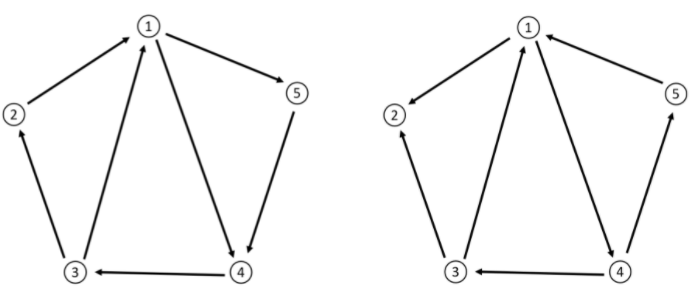
\includegraphics[scale=0.6]{Question1_Figure1.1}\\
		Figure 1.1
	\end{center}
	\begin{enumerate}[(a)]
			% Question 1: Part 1
			\item Are these graphs strongly connected? Explain why or why not.
			% Question 1: Part 2
			\item Are these graphs aperiodic? If a graph is periodic, compute its period.
		\end{enumerate}
\end{enumerate}
\textcolor{gray}{
Answers:
\begin{enumerate}
	\item Consider the following graphs in Figure 1.1
	\begin{enumerate}[(a)]
		% Question 1: Part 1
		\item In Figure 1.1 we see two different directed graphs.  To check if a graph is strongly connected or not a \textit{depth first search} can be done on the graph starting from some node, $x_i$, in set, $X$, of nodes that exists in the graph $G$.  The depth search is a pretty common algorithm the steps through trying to traverse from one node each node that exist. If there exists a path in between any set of nodes that is cyclical then the starting node will be visited twice and we call the graph strongly connected.  As we can see looking at the graph on the left that there exists a path in-between all the nodes that traverses along the outside of the graph.  As for the graph on the right we see that node 2 is only visited and has no edges leaving it so any path that is traversed from node 2 will not fine a path back to node 2.  We can also show this by building an adjacency matrix and analysing where there are columns that are all zeros which would suggest a weakly connected graph.  So we get,
		$\begin{bmatrix} 
			0  & 0  & 0 & 1 & 1 \\
			1  & 0  & 0 & 0 & 0 \\
			1  & 1  & 0 & 0 & 0 \\
			0  & 0  & 1 & 0 & 0 \\
			0  & 0  & 0 & 1 & 0 
		\end{bmatrix}$
and 
		$\begin{bmatrix} 
			0 & 1 & 0 & 1 & 0 \\
			0 & 0 & 0 & 0 & 0 \\
			1 & 1 & 0 & 0 & 0 \\
			0 & 0 & 1 & 0 & 1 \\
			1 & 0 & 0 & 0 & 0 
		\end{bmatrix}$
 as we can see the first matrix shown on the left represents the graph on the left in Figure 1.1 and the second matrix on the right represents the graph on the right in Figure 1.1.  By looking at the first matrix see see that there are no rows with just zeros and this show us that this graph is in fact strongly connected.  As for the graph on the right we can call this graph weakly connected because we can see that row 2 has no edges leaving it.  This suggests that this graph on the right is weakly connected. 
		% Question 1: Part 2
		\item As for checking if the two graphs in Figure 1.1 are aperiodic or not, we can see that although not both graphs are strongly connected, they are both cyclical and their fore have some form of periodicity.  For the graph of the left we see multiple loops of different lengths.  The greatest common denominator (GCD) of each of these lengths is one. So the graph on the left can be considered as aperiodic.  As for the graph on the right, its different loops consists of lengths with a GCD of 3 so the period for this graph on the right is 3.
	\end{enumerate}
\end{enumerate}
}

% Question 2
\begin{enumerate}
	\setcounter{enumi}{1}
	\item Consider the following weighted adjacency matrix in Figure 1.2:
	\begin{center}
		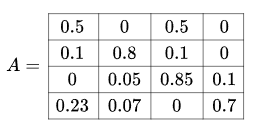
\includegraphics[scale=0.6]{Question2_Figure1.2}\\
		Figure 1.2
	\end{center}
	\begin{enumerate}[(a)]
		% Question 2: Part 1
		\item Is this matrix row-stochastic?
		% Question 2: Part 2
		\item Draw the graph corresponding to this matrix.
		% Question 2: Part 3
		\item Is the graph strongly connected?
		% Question 2: Part 4
		\item Is the graph aperiodic?
	\end{enumerate}
\end{enumerate}
\textcolor{gray}{
Answers:
\begin{enumerate}
	\setcounter{enumi}{1}
	\item Consider the following weighted adjacency matrix in Figure 1.2:
	\begin{enumerate}[(a)]
			% Question 2: Part 1
			\item Yes, the matrix representation in Figure 1.2 does indeed suggest that the graph with weighted edges represented by this matrix is row stochastic.  We can prove this by seeing that there are no negative values in the matrix along with the fact that each weight located inside each individual row adds up to one. So, by adding up each value inside of it's own row we get,
\begin{align*}
	0.5 + 0 + 0.5 + 0  		&= 1		&\text{(Row 1)}\\
	0.1 + 0.8 + 0.1 + 0  	&= 1		&\text{(Row 2)}\\
	0 + 0.05 + 0.85 + 0.1  	&= 1		&\text{(Row 3)}\\
	0.23 + 0.07 + 0 + 0.7 	&= 1		&\text{(Row 4)}\\
\end{align*} 
			% Question 2: Part 2
			\item Drawing of graph represented by matrix in Figure 1.2	is illustrated below in Figure 1.2.2.\\
			\begin{center}
				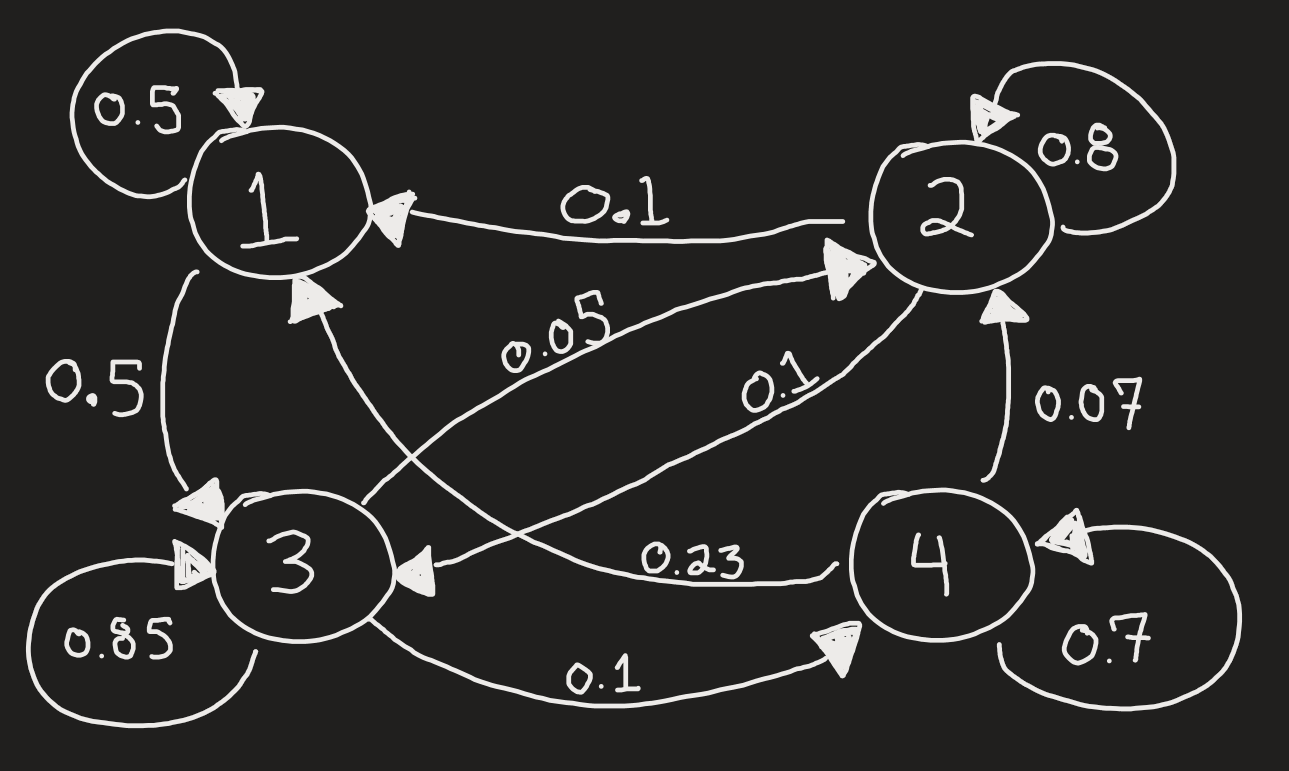
\includegraphics[scale=0.6]{Question2PartB_Figure1.2.2}\\
				Figure 1.2.2
			\end{center}
			% Question 2: Part 3
			\item Yes, by performing the same method used earlier we see that every node has a path that can be traversed from itself to other nodes that will eventually follow back to the original starting node.
			% Question 2: Part 4
			\item We can say that yes this graph is aperiodic as it has multiple places where it can loop on its self as many times as it wants leaving the GCD to be one.
	\end{enumerate}
\end{enumerate}
}

\begin{enumerate}
	\setcounter{enumi}{2}
	% Question 3
	\item Consider the following graph in Figure 1.3
	\begin{center}
		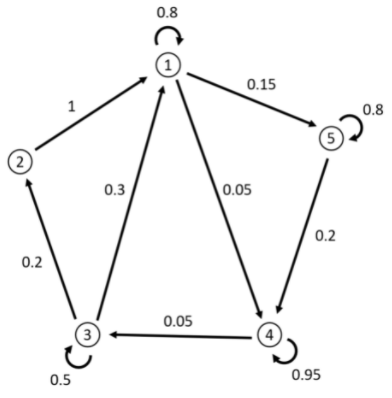
\includegraphics[scale=0.6]{Question3_Figure1.3}\\
		Figure 1.3
	\end{center}
	\begin{enumerate}[(a)]
		% Question 3: Part 1
		\item Write the weighted adjacency matrix corresponding to this graph. Verify that the graph you wrote is row-stochastic.
		% Question 3: Part 2
		\item By hand, using matrix multiplication, perform 1 step of the DeGroot opinion dynamic model on this graph with initial opinions of (1, 1, 0.5, 0, 0).
		% Question 3: Part 3
		\item In the DeGroot opinion dynamics model, which node's initial opinion gets the most weight in society's final opinion? Which node gets the least weight? (it is highly recommended that you use computer code to answer this question).
	\end{enumerate}	
\end{enumerate}
\textcolor{gray}{
Answers:
\begin{enumerate}
	\setcounter{enumi}{2}
	% Question 3
	\item Consider the following graph in Figure 1.3
	\begin{enumerate}[(a)]
		% Question 3: Part 1
		\item We write the weighted graph adjacent matrix as
		$$\begin{bmatrix} 
			0.8  & 0.0  & 0.0  & 0.05 & 0.15 \\
			1.0  & 0.0  & 0.0  & 0.0   & 0.0 \\
			0.3  & 0.2  & 0.5  & 0.0   & 0.0 \\
			0.0  & 0.0  & 0.05 & 0.95 & 0.0 \\
			0.0  & 0.0  & 0.0  & 0.2  & 0.8 \\
		\end{bmatrix}$$
then by adding up all the values for each row we get,
		\begin{align*}
			0.8 + 0.0 + + 0.0 + 0.05 + 0.15  	&= 1		&\text{(Row 1)}\\
			1.0 + 0.0 + 0.0 + 0.0 + 0.0 		&= 1		&\text{(Row 2)}\\
			0.3 + 0.2 + 0.5 + 0.0 + 0.0  		&= 1		&\text{(Row 3)}\\
			0.0 + 0.0 + 0.05 + 0.95 + 0.0		&= 1		&\text{(Row 4)}\\
			0.0 + 0.0 + 0.0 + 0.2 + 0.8		&= 1		&\text{(Row 5)}\\
		\end{align*} 
As we can see that there are no negative values in the matrix and all the values in each row all add up to one, so the matrix is row-stochastic. 
		% Question 3: Part 2
		\item 	Assuming the value of the initial opinions given represent a column vector, we can use this vector to then perform matrix multiplication on the two matrices,  \\ \\
		% First Column
		$\begin{bmatrix} 
			0.8  & 0.0  & 0.0  & 0.05 & 0.15 \\
		\end{bmatrix}$ 
		x
		$\begin{bmatrix} 
			1  \\  1  \\ 0.5  \\ 0.0 \\ 0.0 \\
		\end{bmatrix}$
		=
		0.8(1)+0.0(1)+0.0(0.5)+0.05(0.0)+0.15 (0.0)=0.8\\ 
		% Second Column
		$\begin{bmatrix} 
			1.0  & 0.0  & 0.0  & 0.0   & 0.0 \\
		\end{bmatrix}$
		x
		$\begin{bmatrix} 
			1  \\  1  \\ 0.5  \\ 0.0 \\ 0.0 \\
		\end{bmatrix}$
		=
		1.0(1)+0.0(1)+0.0(0.5)+0.0(0.0)+0.0(0.0)=1\\ 
		% Third Column
		$\begin{bmatrix} 
			0.3  & 0.2  & 0.5  & 0.0   & 0.0 \\
		\end{bmatrix}$ 
		x
		$\begin{bmatrix} 
			1  \\  1  \\ 0.5  \\ 0.0 \\ 0.0 \\
		\end{bmatrix}$
		=
		0.3(1)+0.2(1)+0.5(0.5)+0.0(0.0)+0.0(0.0)=0.75\\ 
		% Fourth Column
		$\begin{bmatrix} 
			0.0  & 0.0  & 0.05 & 0.95 & 0.0 \\
		\end{bmatrix}$
		x
		$\begin{bmatrix} 
			1  \\  1  \\ 0.5  \\ 0.0 \\ 0.0 \\
		\end{bmatrix}$
		=
		0.0(1)+0.0(1)+0.05(0.5)+0.95(0.0)+0.0(0.0)=0.025\\ 
		% Fifth Column
		$\begin{bmatrix} 
			0.0  & 0.0  & 0.0  & 0.2  & 0.8 
		\end{bmatrix}$
		x
		$\begin{bmatrix} 
			1  \\  1  \\ 0.5  \\ 0.0 \\ 0.0 \\
		\end{bmatrix}$
		=
		0.0(1)+0.0(1)+0.0(0.5)+0.2(0.0)+0.8(0.0)=0.0\\ \\  
So we have are opinion vector at the first time step, $t=1$.  This gives us,\\
		$x(t) \ = \ $
		$\begin{bmatrix} 
			0.8  \\ 1  \\ 0.75  \\ 0.025 \\ 0.0 \\
		\end{bmatrix}$
		% Question 3: Part 3
		\item In this example of a  DeGroot opinion dynamics model, to find the node with the most influential opinion in the graph we can use the graph's adjacent matrix, $A$, to  calculate $\bar{A}$ which will be equal to be the matrix squared, $A^2$.  So we get,\\
		$\begin{bmatrix} 
			0.8  & 0.0  & 0.0  & 0.05 & 0.15 \\
			1.0  & 0.0  & 0.0  & 0.0   & 0.0 \\
			0.3  & 0.2  & 0.5  & 0.0   & 0.0 \\
			0.0  & 0.0  & 0.05 & 0.95 & 0.0 \\
			0.0  & 0.0  & 0.0  & 0.2  & 0.8 
		\end{bmatrix}$
		x
		$\begin{bmatrix} 
			0.8  & 0.0  & 0.0  & 0.05 & 0.15 \\
			1.0  & 0.0  & 0.0  & 0.0   & 0.0 \\
			0.3  & 0.2  & 0.5  & 0.0   & 0.0 \\
			0.0  & 0.0  & 0.05 & 0.95 & 0.0 \\
			0.0  & 0.0  & 0.0  & 0.2  & 0.8 
		\end{bmatrix}$\\
                   $ \bar{A} \ = \ $
		$\begin{bmatrix} 
			0.64  	& 0.0   	& 0.00025 	& 0.11755    & 0.24 \\
			0.8    	& 0.0   	& 0.0   	& 0.05  	& 0.15\\
			0.59  	& 0.1  	& 0.25 	& 0.015   	& 0.045 \\
			0.015 	& 0.01   	& 0.00725   	& 0.9025 	& 0.0 \\
			0.0    	& 0.0   	& 0.01   	& 0.035     	& 0.64 
		\end{bmatrix}$\\
We can see that the opinion that is the most weighted and influential on the graph is node 4 because it has a value of 0.95 and self loops on it's self.  We also showed in class that by finding the matrix squared, we can look at the product of the matrix multiplication to evaluate such relationships between nodes.  We can see that 0.95 in the fourth column has the greatest value. It also loops on its self and will continue to be influence its self in this aspect.  We also look at the product matrix to see that the column for node 4 seems to converge to a larger value. These two factors are enough information for us to see that the node with the most influence would be node 4.\\
 As for the node with the least influence on the entire graph, node 2 seems to not be listened to at all and their fore is the least influential node on the graph. 
	\end{enumerate}	
\end{enumerate}
}

% Question 4
\begin{enumerate}
	\setcounter{enumi}{3}
	\item Consider again the graph from problem 2 (Figure 1.2).
	\begin{enumerate}[(a)]
		% Question 4: Part 1
		\item By hand, using matrix multiplication, perform 1 step of the Friedkin-Johnsen opinion dynamic model on this graph with initial opinions of (1, 1, 0.5, 0) and lambda values of (0.9, 0.1, 0.8, 1).
		% Question 4: Part 2
		\item As we discussed in class, in the Friedkin-Johnsen model, nodes usually have differing opinions even after a long time. Keeping the lambda values from part A, experiment with this graph and try to find an assignment of initial opinions that results in the most different limiting opinions. That is, what equilibrium on this graph can have the most disagreement out of all equilibria? You will likely want to use compute code to solve this problem. Full credit is possible if you show understanding and effort; I will award 1 bonus point if you can show that your answer is the most disagreement possible.
	\end{enumerate}
\end{enumerate}
\textcolor{gray}{
Answers:
\begin{enumerate}
	\setcounter{enumi}{3}
	\item Consider again the graph from problem 2 (Figure 1.2).
	\begin{enumerate}[(a)]
		% Question 4: Part 1
		\item To begin we first initialize a matrix from question two as well as the original opinion listed for this question, (1, 1, 0.5, 0).  We can then use the listed lambda values for this question, (0.9, 0.1, 0.8, 1), to create a diagonal matrix, $\Lambda$ like so,\\
		\begin{center}
		$\Lambda \ = \ $
		$\begin{bmatrix} 
			0.9 & 0.0  & 0.0 & 0.0 \\
			0.0 & 0.1  & 0.0 & 0.0 \\
			0.0 & 0.0  & 0.8 & 0.0 \\
			0.0 & 0.0  & 0.0 & 0.1 \\
		\end{bmatrix}$\\
		\end{center}
We then take the inner product of the diagonal and adjacent matrix to get,\\
		$\begin{bmatrix} 
			0.9 & 0.0  & 0.0 & 0.0 \\
			0.0 & 0.1  & 0.0 & 0.0 \\
			0.0 & 0.0  & 0.8 & 0.0 \\
			0.0 & 0.0  & 0.0 & 0.1 \\
		\end{bmatrix}$
		.
		$\begin{bmatrix} 
			0.5  & 0.0  	& 0.5   & 0.0 \\
			0.1  & 0.8  	& 0.1   & 0.0 \\
			0.0  & 0.05   & 0.85 & 0.1 \\
			0.23 & 0.07  & 0.0 & 0.7 \\ 
		\end{bmatrix}$ \\ \\
		% First Row
		0.9(0.5)  + 0.0(0.1) + 0.0(0.0) + 0.0(0.23) = 0.45  \\
		0.9(0.0)  + 0.0(0.8) + 0.0(0.05) + 0.0(0.07) = 0.0  \\
		0.9(0.5)  + 0.0(0.1) + 0.0(0.85) + 0.0(0.1) = 0.45  \\
		0.9(0.0)  + 0.0(0.0) + 0.0(0.1) + 0.0(0.7) = 0.0 \\
		% Second Row
		0.0(0.5)  + 0.1(0.1) + 0.0(0.0) + 0.0(0.23) = 0.01 \\
		0.0(0.0)  + 0.1(0.8) + 0.0(0.05) + 0.0(0.07) = 0.08 \\
		0.0(0.5)  + 0.1(0.1) + 0.0(0.85) + 0.0(0.1) = 0.01 \\
		0.0(0.0)  + 0.1(0.0) + 0.0(0.1) + 0.0(0.7) = 0.0 \\
		% Third Row
		0.0(0.5)  + 0.0(0.1)  + 0.8(0.0) + 0.0(0.23) = 0.0\\
		0.0(0.0)  + 0.0(0.8)  + 0.8(0.05) + 0.0(0.07) = 0.04\\
		0.0(0.5)  + 0.0(0.1)  + 0.8(0.85) + 0.0(0.1) = 0.68\\
		0.0(0.0)  + 0.0(0.00)  + 0.8(0.1) + 0.0(0.7) = 0.08\\
		% Fourth Row
		0.0(0.5)  + 0.0(0.1)  + 0.0(0.0) + 0.1(0.23) = 0.023\\
		0.0(0.0)  + 0.0(0.8)  + 0.0(0.05) + 0.1(0.07) = 0.007\\
		0.0(0.5)  + 0.0(0.1)  + 0.0(0.85) + 0.1(0.1) = 0.0\\
		0.0(0.0)  + 0.0(0.00)  + 0.0(0.1) + 0.1(0.7) = 0.07\\
		=
		$\begin{bmatrix} 
			0.45  & 0.0  	& 0.45   	& 0.0 \\
			0.01  & 0.08  	& 0.01   	& 0.0 \\
			0.0    & 0.04   	& 0.68 	& 0.08 \\
			0.023  & 0.007  	& 0.0 	 & 0.07 \\ 
		\end{bmatrix}$ \\ \\
Once we have this matrix we can then take the inner product of this matrix along with the stored vector matrix values from the previous time step.  So we get, \\
		$\begin{bmatrix} 
			0.45  & 0.0  	& 0.45   	& 0.0 \\
			0.01  & 0.08  	& 0.01   	& 0.0 \\
			0.0    & 0.04   	& 0.68 	& 0.08 \\
			0.023  & 0.007  	& 0.0 	 & 0.07 \\ 
		\end{bmatrix}$
		.
		$\begin{bmatrix} 
			x_{1}(t-1)  \\ x_{2}(t-1)  \\ x_{3}(t-1)   \\ x_{4}(t-1) \\
		\end{bmatrix}$\\
Since in this case this is our first time step we simply take the initial opinion. So we get, \\
		$\begin{bmatrix} 
			0.45  & 0.0  	& 0.45   	& 0.0 \\
			0.01  & 0.08  	& 0.01   	& 0.0 \\
			0.0    & 0.04   	& 0.68 	& 0.08 \\
			0.023  & 0.007  	& 0.0 	 & 0.07 \\ 
		\end{bmatrix}$
		.
		$\begin{bmatrix}
			0.9 \\ 0.1 \\ 0.8 \\ 0.1 
		\end{bmatrix}$\\
		0.45(0.9)  + 0.0(0.1)  + 0.45(0.8) + 0.0(0.1) = 0.765\\
		0.01(0.9)  + 0.08(0.1) + 0.01(0.8)   + 0.0(0.1) = 0.025\\
		0.0(0.9)    + 0.04(0.1) + 0.68(0.8) 	+ 0.08(0.1) = 0.0556\\
		0.023(0.9)  + 0.007(0.1) + 0.0(0.8) + 0.07(0.1) = 0.0284\\ 
		=
		$\begin{bmatrix}
			0.765 \\ 0.025 \\ 0.0556 \\ 0.0284
		\end{bmatrix}$\\
Once we have taken the vector matrix values from the previous time step. We use them to calculate the inner products for the current time step. We can then continue onto the second part of the equation. So we add this to the inverse of the inner product of the original opinion and then the inner product of this and the adjacent matrix. So for the second part we get something like this,\\
\begin{center}
$
	\sum^{t-i}_{i=0} = (1-\Lambda) A 
$  
\end{center}
Since our last time step values are our $\Lambda$ values we see that the inverse of this inner product would look something like,\\
		$\begin{bmatrix} 
			0.1 & 0.0  	& 0.0 & 0.0 \\
			0.0 & 0.9  	& 0.0 & 0.0 \\
			0.0 & 0.0   	& 0.2 & 0.00 \\
			0.0 & 0.0  	& 0.0  & 0.9 \\ 
		\end{bmatrix}$\\
Which we then use to take another inner product with the previous stored executed time steps to get,\\
		$\begin{bmatrix} 
			0.1 & 0.0  	& 0.0 & 0.0 \\
			0.0 & 0.9  	& 0.0 & 0.0 \\
			0.0 & 0.0   	& 0.2 & 0.00 \\
			0.0 & 0.0  	& 0.0  & 0.9 \\ 
		\end{bmatrix}$
		.	
		$\begin{bmatrix} 
			0.9 \\ 0.1 \\ 0.8 \\ 0.1
		\end{bmatrix}$\\
		% First Row
		0.1(0.9)  + 0.0(0.1) + 0.0(0.8) + 0.0(0.1) = 0.09  \\
		% Second Row
		0.0(0.9)  + 0.9(0.1) + 0.0(0.8) + 0.0(0.1) = 0.09 \\
		% Third Row
		0.0(0.9)  + 0.0(0.1)  + 0.2(0.8) + 0.0(0.1) = 0.16 \\
		% Fourth Row
		0.0(0.9)  + 0.0(0.1)  + 0.0(0.8) + 0.9(0.1) = 0.09 \\ \\
		$\begin{bmatrix} 
			0.09  \\ 0.09  \\ 0.16 \\ 0.09 \\
		\end{bmatrix}$ \\ \\
We then sum this value with the value calculated early and save this information for future iterations,\\
		$\begin{bmatrix} 
			0.765 \\ 0.025 \\ 0.0556 \\ 0.0284
		\end{bmatrix}$
		+
		$\begin{bmatrix} 
			0.09  \\ 0.09  \\ 0.16 \\ 0.09 \\
		\end{bmatrix}$
		=
		$\begin{bmatrix} 
		0.855 \\ 0.115 \\ 0.716 \\ 0.1184
		\end{bmatrix}$
		% Question 4: Part 2
		\item Although not many values or simulations were ran on this model it seemed apparent that the more the original opinions differed the more they seemed to diverge from each other opinions. 
	\end{enumerate}
\end{enumerate}
}
\end{document}
